\documentclass{article}
\usepackage{v-equation}
\vgeometry

\begin{document}
\color{white}
\def\gdrive{https://drive.google.com/drive/folders/14S0LI9yfRNtN-hgkQcDEnv49WdEBDES_?usp=share_link}
\vtitle[Possible paths in a uniform magnetic field]

\begin{itemize}
\item Projected from inside and there's no boundary restriction
\begin{center}
\begin{tikzpicture}
	[thick]
\def\r{2.5}
	\foreach \x in {-1, 0, ..., 7}{
		\foreach \y in {-1, 0, ..., 7}{
			\node at (\x, \y){$\times$};
		}
	} 
	\tzcoor*(5.5, 3)(O){$q_0$}[r](7pt)
	\tzcoor($(O)+(-\r,0)$)(C)
	
	\tzline+[->](O)(0, 1){$\vec{v}$}[a]
	\tzline+[->](O)(-1, 0){$\vec{F}_m$}[l]
	\tzarc[-->--=0.5, dashed](C)(0:360:\r)
	
\end{tikzpicture}
\end{center}

\pagebreak

\item Projected from outside at $90^\circ$ with respect to the boundary line
\begin{center}
\begin{tikzpicture}
	[thick]
\def\a{90}
\def\r{3}
	\foreach \x in {0, 1, ..., 6}{
		\foreach \y in {-4,-3, ..., 4}{
			\node at (\x, \y){$\times$};
		}
	} 
	
	\tzcoor(-\r*cos{\a}, 0)(O)
	\tzcoor*($(O)+(\r*cos{\a}, -\r*sin{\a})$)(q){$q_0$}[bl](7pt)
	\tzcoor*($(O)+(\r*cos{\a}, \r*sin{\a})$)(q'){$q_0$}[ar](7pt)
	
	\tzline+[->](q)(sin{\a}, cos{\a}){$\vec{v}$}[ar]
	\tzline+[->](q)(-cos{\a}, sin{\a}){$\vec{F}_m$}[al]
	
	\tzline+[->](q')(-sin{\a}, cos{\a}){$\vec{v}$}[al]
	\tzline+[->](q')(-cos{\a}, -sin{\a}){$\vec{F}_m$}[bl]
	
	\tzarc[dashed](O)(-\a:\a:\r)
	\tzline[dashed](O)($(O)+(\r*cos{\a}, -\r*sin{\a})$)
	\tzline[dashed](O)($(O)+(\r*cos{\a}, \r*sin{\a})$)
	
\end{tikzpicture}
\end{center}

\pagebreak

\item Projected from outside at acute angle with respect to the boundary line
\begin{center}
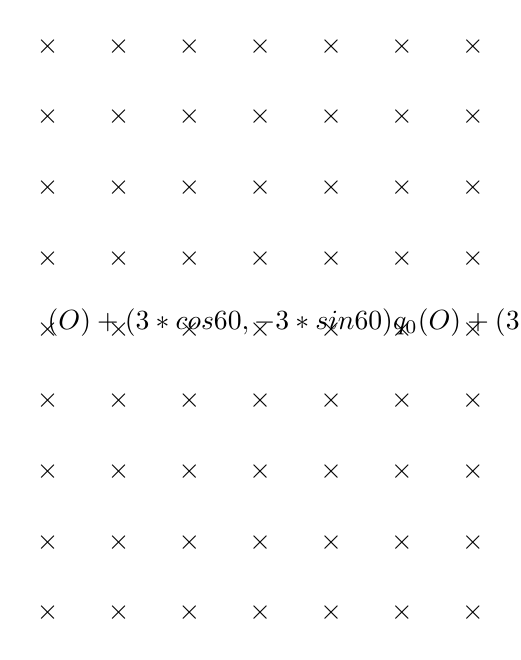
\begin{tikzpicture}
[thick, scale=0.9]
\def\a{60}
\def\r{3}
	\foreach \x in {0, 1, ..., 6}{
		\foreach \y in {-4, -3, ..., 4}{
			\node at (\x, \y){$\times$};
		}
	} 
	
	\tzcoor(-\r*cos{\a}, 0)(O)
	\tzcoor*($(O)+(\r*cos{\a}, -\r*sin{\a})$)(q){$q_0$}[bl](7pt)
	\tzcoor*($(O)+(\r*cos{\a}, \r*sin{\a})$)(q'){$q_0$}[ar](7pt)
	
	\tzline+[->](q)(sin{\a}, cos{\a}){$\vec{v}$}[ar]
	\tzline+[->](q)(-cos{\a}, sin{\a}){$\vec{F}_m$}[al]
	
	\tzline+[->](q')(-sin{\a}, cos{\a}){$\vec{v}$}[al]
	\tzline+[->](q')(-cos{\a}, -sin{\a}){$\vec{F}_m$}[bl]
	
	\tzarc[dashed](O)(-\a:\a:\r)
	\tzline[dashed](O)($(O)+(\r*cos{\a}, -\r*sin{\a})$)
	\tzline[dashed](O)($(O)+(\r*cos{\a}, \r*sin{\a})$)
	
\end{tikzpicture}
\end{center}

\pagebreak

\item Projected from outside at obtuse angle with respect to the boundary line
\begin{center}
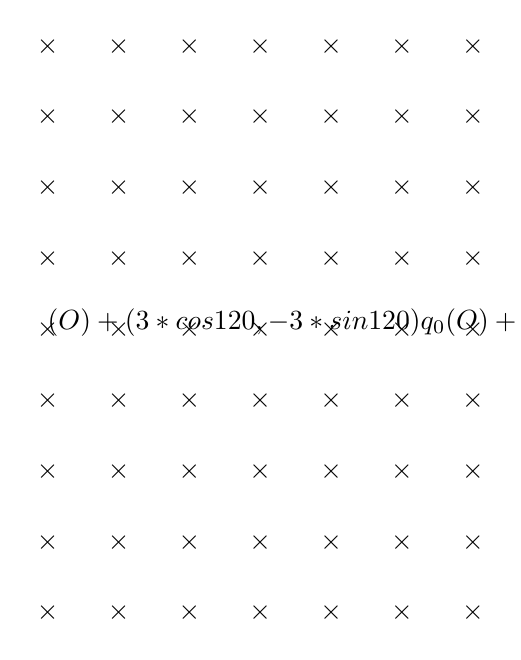
\begin{tikzpicture}
[thick, scale=0.9]
\def\a{120}
\def\r{3}
	\foreach \x in {0, 1, ..., 6}{
		\foreach \y in {-4, -3, ..., 4}{
			\node at (\x, \y){$\times$};
		}
	} 
	
	\tzcoor(-\r*cos{\a}, 0)(O)
	\tzcoor*($(O)+(\r*cos{\a}, -\r*sin{\a})$)(q){$q_0$}[bl](7pt)
	\tzcoor*($(O)+(\r*cos{\a}, \r*sin{\a})$)(q'){$q_0$}[ar](7pt)
	
	\tzline+[->](q)(sin{\a}, cos{\a}){$\vec{v}$}[ar]
	\tzline+[->](q)(-cos{\a}, sin{\a}){$\vec{F}_m$}[al]
	
	\tzline+[->](q')(-sin{\a}, cos{\a}){$\vec{v}$}[al]
	\tzline+[->](q')(-cos{\a}, -sin{\a}){$\vec{F}_m$}[bl]
	
	\tzarc[dashed](O)(-\a:\a:\r)
	\tzline[dashed](O)($(O)+(\r*cos{\a}, -\r*sin{\a})$)
	\tzline[dashed](O)($(O)+(\r*cos{\a}, \r*sin{\a})$)
	
\end{tikzpicture}
\end{center}
\end{itemize}
\vspace*{\fill}



\pagebreak

\vspace*{\fill}
\begin{center}
    \fbox{\qrcode[height=2cm]{\gdrive}}
\end{center}
\vspace*{\fill}
\end{document}
